\chap{The runtime}{runtime}
\section{Notes}

There are multiple, possibly orthogonal issues.  Limit checks and garbage
collections are a little overloaded in their roles, because they also
support preemptive thread switching and interrupt handling.  Forcing
frontier to be 0 and hitting a limit check (even a zero byte limit check)
will invoke the GC, which will switch to the pending thread.

Recall that a limit check with bytes = 0 really means a check for LIMIT\_SLOP
bytes (currently LIMIT\_SLOP = 512).

\section{Bootstrap}

\figBegin
\centerline{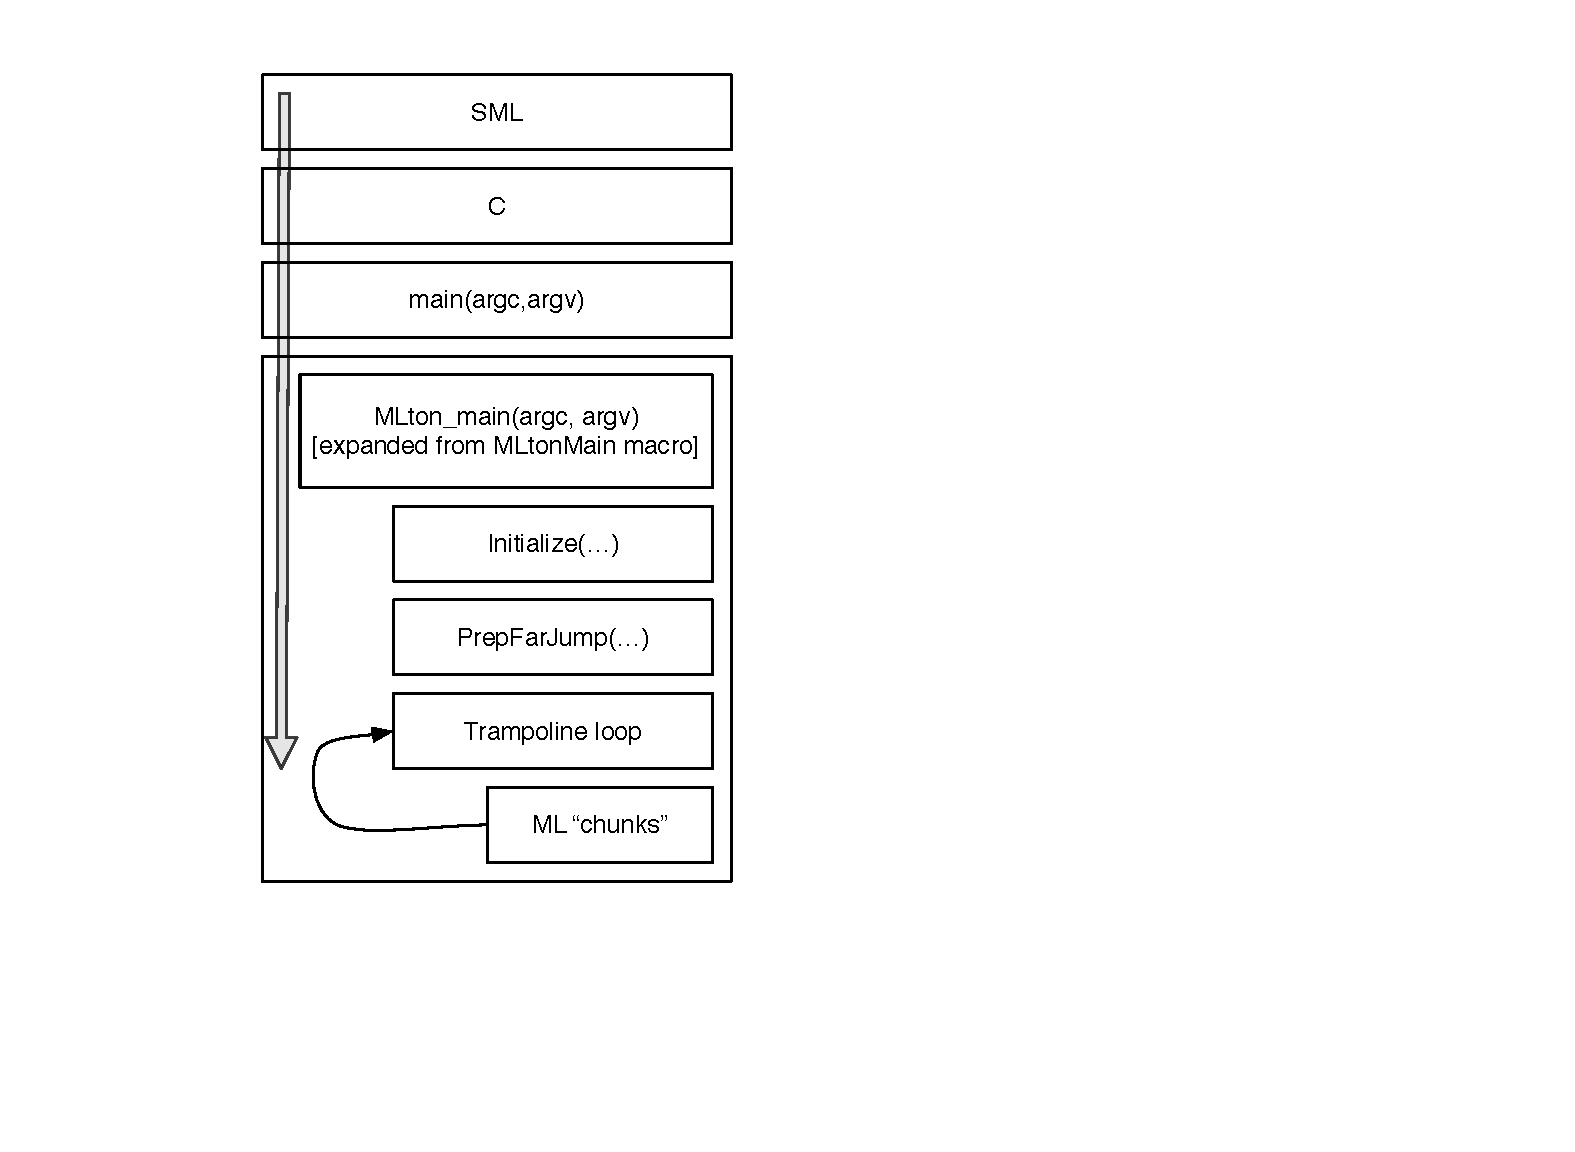
\epsfig{file=runtime-bootstrap-overview.pdf,width=2.0in}}
\figEnd{Runtime overview}{rtoverview}
       
When you compile your SML code, it is translated to machine code using one of several backends. For an in-depth description of how SML is compiled and optimized refer to~\cite{leibig:mlton-llvm-backend}. We will look at the C translation of a trivial SML program starting at the backend once all optimization phases have completed. The trivial SML program is a single statement: \texttt{val a = 2}

When reading this section of the guide, it will be useful to save the above statement as "test.sml" and then compile that using "mlton -keep g test.sml" so that you can refer to the intermediate files "test.0.c" "test.1.c" and "test.2.c"

Refer to Figure~\ref{figure:rtoverview} for an overview of how the compiler emits C code given SML code, and how control flows through the bootstrap process of the emitted code.

 
The emitted C code bootstrap at the bottom of "test.0.c" looks like this:

\begin{minipage}{\linewidth}
\lstset{language=C}\begin{lstlisting}
MLtonMain (8, 0x7CB29B69, 136, TRUE, PROFILE_NONE, FALSE, 0, 218)
int main (int argc, char* argv[]) {
    return (MLton_main (argc, argv));
}
\end{lstlisting}
\end{minipage}

\noindent and contains a \texttt{main} routine that calls \texttt{MLton\_main} which is created when the \texttt{MLtonMain} macro is expanded. 
\texttt{MLtonMain} is defined in \texttt{include/c-main.h} as a macro:

\begin{minipage}{\linewidth}
\lstset{language=C}\begin{lstlisting}
#define MLtonMain(al, mg, mfs, mmc, pk, ps, mc, ml)	
\end{lstlisting}
\end{minipage}

and ultimately calls the routine \texttt{MLton\_main (int argc, char* argv[])} which 

The parameters to the \texttt{MLtonMain} macro are:

\setlist[description]{leftmargin=!,labelindent=\parindent,labelwidth=1.5cm}

\begin{description}
\item[al] alignment width (\texttt{-align})
\item[mg] a magic random number used for saving/restoring the world. This number is generated at compile time by \texttt{mlton/codegen/c-codegen/c-codegen.fun} and allows the application to save and restore its state (\htmladdnormallink{MLtonWorld}{http://mlton.org/MLtonWorld})
\item[mfs] the maximum frame size
\item[mmc] whether or not the mutator marks cards. This is an optimization strategy used by the generational GC.
\item[pk] the kind of profiling to perform (compile time option)
\item[ps] whether stack profiling is enabled (\texttt{-profile-stack})
\item[mc] the number of the first chunk to jump to
\item[ml] the function number in the chunk to jump to
\end{description}

The first six of these parameters are passed to \texttt{Initialize} (defined in \texttt{include/common-main.h}) while the final two (mc and ml) are passed to \texttt{PrepFarJump} (defined in \texttt{include/c-common.h}). 
\texttt{Initialize} sets variables in the \texttt{gcState} structure and then calls \texttt{MLton\_init(argc, argv, \&gcState)}.



\texttt{MLton\_init} (\texttt{runtime/platform.c}) initializes the posix environment, the GC and processes the runtime command line arguments.  Once \texttt{Initialize} completes, \texttt{MLton\_main} continues and calls \texttt{PrepFarJump} to prepare to jump to the first chunk of the SML program. Alternatively, it will restore the saved world and restart from where the saved program left off. Finally, \texttt{MLton\_main} goes into an infinite loop, jumping from chunk to chunk as the SML program executes.

Jumping between chunks is known as trampolining and this is done to avoid mapping highly recursive SML functions directly to C functions as this would exhaust the C stack (see \S2.2.4 of~\cite{leibig:mlton-llvm-backend}). Trampolining involves selecting a chunk from the \texttt{cont} struct and then calling to that address (pointer). You will notice that, in our example above, \texttt{mc} is set to 0 and \texttt{ml} is set to 218. That means that \texttt{PrepFarJump} will select chunk 0 to execute and will set the next function within chunk zero to 218. 

So walking through this, \texttt{SetFarJump(0, 218)} will result in 

\begin{minipage}{\linewidth}
\lstset{language=C}\begin{lstlisting}
cont.nextChunk = (void *)Chunk0;
nextFun = 218;
\end{lstlisting}
\end{minipage}

The \texttt{Chunk0} symbol is declared in "test.0.c" via the \texttt{DeclareChunk (0)} line. This is a macro that expands to 

\begin{minipage}{\linewidth}
\lstset{language=C}\begin{lstlisting}
PRIVATE struct cont Chunk0(void);
\end{lstlisting}
\end{minipage}

The actual \texttt{Chunk0} routine is defined in "test.2.c" via the line \texttt{Chunk (0)} which is another macro (defined in \texttt{include/c-chunk.h} that expands to:

\begin{minipage}{\linewidth}
\lstset{language=C}\begin{lstlisting}
	
        DeclareChunk(0) {
                struct cont cont;
                Pointer frontier;
                uintptr_t l_nextFun = nextFun; // remember this is 218
                Pointer stackTop;
\end{lstlisting}
\end{minipage}

Where \texttt{DeclareChunk} is, you guessed it, a macro (defined in \texttt{include/c-common.h}) and so results in the above expanding to:


\begin{minipage}{\linewidth}
\lstset{language=C}\begin{lstlisting}
PRIVATE struct cont Chunk0(void) {
                struct cont cont;
                Pointer frontier;
                uintptr_t l_nextFun = nextFun; // remember this is 218
                Pointer stackTop;
\end{lstlisting}
\renewcommand{\lstlistingname}{Code}
\end{minipage}

And so we finally have our \texttt{Chunk0} routine which is what we set \texttt{chunk.nextChunk} to above if you recall.





Given the above, the trampoline section of \texttt{MLton\_main} (again, in \texttt{include/c-main.h}) will call


\begin{minipage}{\linewidth}
\lstset{language=C}\begin{lstlisting}
cont=(*(struct cont(*)(void))cont.nextChunk)(); 
\end{lstlisting}
\end{minipage}

We will see, as we fully expand \texttt{Chunk0} how it ultimately returns a \texttt{cont} structure to allow us to trampoline to the next chunk. Also, we will see how each chunk routine is a large \texttt{switch} statement indexed by nextFun and so, architecturally, MLton aggregates SML functions into large C-functions where each SML function is one of the cases in the switch statement. This is how MLton minimizes the growth of the C-stack.

Continuing on, we are now in the \texttt{Chunk0} routine which we see, from examining "test.2.c" continues past the \texttt{Chunk (0)} line as such:

\begin{minipage}{\linewidth}
\lstset{language=C}\begin{lstlisting}
Chunk (0)
        CPointer Q_0;
        CPointer Q_1;
        CPointer Q_2;
	.
	.
	.
ChunkSwitch (0)
case 5:
L_9:
        Push (-8);
	.
	.
	.
case 218:
        G(Word32, 0) = CPointer_lt (O(CPointer, GCState, 40), StackTop);
        BNZ (G(Word32, 0), L_8);
        G(Word64, 0) = CPointer_diff (O(CPointer, GCState, 1360), Frontier);
        G(Word32, 1) = WordU64_lt (G(Word64, 0), (Word64)(0x1090ull));
        BNZ (G(Word32, 1), L_8);
        goto L_2;
	.
	.
	.
EndChunk
\end{lstlisting}
\end{minipage}

Examining this routine, let's first look at the bottom \texttt{EndChunk} which is a macro (defined in \texttt{include/c-chunk.h}) and expands to:

\begin{minipage}{\linewidth}
\lstset{language=C}\begin{lstlisting}
                default:
                        /* interchunk return */
                        nextFun = l_nextFun;
                        cont.nextChunk = (void*)nextChunks[nextFun];
                        leaveChunk:
                                FlushFrontier();
                                FlushStackTop();
                                return cont;
                    } /* end switch (l_nextFun) */
                } /* end while (1) */
        } /* end chunk */	
\end{lstlisting}
\end{minipage}

This results in \texttt{nextFun} being set to the next function in the switch statement to execute and then it sets \texttt{cont.nextChunk} to the next chunk (if we need to switch between C functions) and finally it flushes some registers and returns. Note the label \texttt{leaveChunk} allows SML functions to jump out of the C function. The "end while (1)" refers to a while statement in the macro \texttt{ChunkSwitch} which we will now look at, before bringing this all together into a macro-less C fragment.
